\section{Materials and methods}\label{sec:mvtraits-methods}

\subsection{Trait data}

Foliar trait data for this analysis comes from the TRY global traits database (Kattge et al.~2011). \nocite{kattge_try_2011}
We focused our research on seven foliar traits:
Leaf longevity (months),
specific leaf area (SLA, m$^2$ kg$^{-1}$),
leaf nitrogen content ($N_{\mass}$, mg N g$^{-1}$ or $N_{\area}$, g m$^{-2}$),
leaf phosphorus content ($P_{\mass}$, mg P g$^{-1}$ or $P_{\area}$, g m$^{-2}$),
leaf dark respiration at 25°C ($R_{d,\mass}$, µmol g$^{-1}$ s$^{-1}$, or $R_{d,\area}$, µmol m$^{-2}$ s$^{-1}$),
maximum Rubisco carboxylation rate at 25°C ($V_{c,\max,\mass}$, µmol g$^{-1}$ s$^{-1}$, or $V_{c,\max,\area}$, µmol m$^{-2}$ s$^{-1}$),
and maximum electron transport rate at 25°C ($J_{\max,\mass}$, µmol g$^{-1}$ s$^{-1}$, or $J_{\max,\area}$, µmol m$^{-2}$ s$^{-1}$).
For $V_{c,\max}$, we only used values already reported in TRY as being at 25°C.
For $R_{d}$, we normalized the values to 25°C based on reported leaf temperature values following the same methods as Atkin et al.~(2015). \nocite{atkin_global_2015}
For $J_{\max}$, we normalized the values to 25°C based on reported leaf temperature values using the temperature response function described in Kattge \& Knorr (2007, Equation 1 therein). \nocite{kattge_2007_temperature}
To avoid potential artifacts caused by different trait normalization, we performed analyses separately for both mass- and area-normalized traits~\cite{osnas_global_2013,lloyd_les}.
We restricted our analysis to TRY data that have been quality-controlled and for which adequate species information was provided for functional type classification (see Kattge et al.~2011).\nocite{kattge_try_2011}

Although the light- and CO2-saturated photosynthetic rate ($A_{\max}$) was an important trait in previous studies, we did not include it in our study for two reasons.
First of all, data on raw photosynthetic rates are highly sensitive to measurement methodology and environmental conditions, which were generally inconsistent or unavailable in TRY\@.
Second, $A_{\max}$ is not a good measure of photosynthetic capacity because it integrates over variability in many physiologically independent traits such as $V_{c,\max}$, $J_{\max}$, and stomatal conductance, and is therefore not used in vegetation models as a photosynthetic parameter~\cite{Ali_2015}.

Following past studies~\cite{wright_worldwide_2004,wright_assessing_2005,onoda_2011_global,diaz_global_2016}, we log-transformed all trait values to correct for their strong right-skewness.

\subsection{Plant functional types}

\begin{longtable}[]{@{}ccc@{}}
\caption{\label{tab:pfts}Names, labels, and species counts for plant
functional types (PFTs) used in this analysis.}\tabularnewline
\toprule
Label & PFT & Number of species\tabularnewline
\midrule
\endfirsthead
\toprule
Label & PFT & Number of species\tabularnewline
\midrule
\endhead
BlETr & Broadleaf Evergreen Tropical & 1229\tabularnewline
BlETe & Broadleaf Evergreen Temperate & 363\tabularnewline
BlDTr & Broadleaf Deciduous Tropical & 286\tabularnewline
BlDTe & Broadleaf Deciduous Temperate & 345\tabularnewline
BlDBo & Broadleaf Deciduous Boreal & 62\tabularnewline
NlETe & Needleleaf Evergreen Temperate & 130\tabularnewline
NlEBo & Needleleaf Evergreen Boreal & 30\tabularnewline
NlD & Needleleaf Deciduous & 19\tabularnewline
ShE & Shrub Evergreen & 1120\tabularnewline
ShDTe & Shrub Deciduous Temperate & 330\tabularnewline
ShDBo & Shrub Deciduous Boreal & 94\tabularnewline
C3GAr & C3 Grass Arctic & 157\tabularnewline
C3GTe & C3 Grass Temperate & 624\tabularnewline
C4G & C4 Grass & 255\tabularnewline
\bottomrule
\end{longtable}

We assigned each species to a unique plant functional type (PFT) following the scheme in the Community Land Model~\cite[CLM4.5,][]{clm45_note}; Table~\ref{tab:pfts}, Fig.~\ref{fig:mvtraits-fig1}. %TODO: Table
We obtained categorical data on growth form, leaf type, phenology, and photosynthetic pathway from the TRY database.
Where species attributes disagreed between datasets (e.g., categorized as a shrub in one dataset but a tree in another), we assigned the attribute that was observed most frequently between the datasets (e.g., if five datasets say ``shrub'' but only one says ``tree'', we would classify it as a shrub).
Where species lacked data on certain attributes, we assigned those attributes based on higher order phylogeny where appropriate (e.g., *Poaceae* family are usually grasses, *Larix spp.* are deciduous needleleaved trees) or otherwise omitted the species from our analyses.
For biome specification, we collected all latitude and longitude data for each species,
matched these data to 30 second ($\sim1$ km$^{2}$) mean annual temperature ($AMT$, averaged 1970--2000) data from WorldClim-2~\cite{worldclim},
calculated the mean AMT for all sites at which that species was observed,
and then binned these species based on the following cutoffs: boreal/arctic ($AMT \leq 5^\circ C$), temperate ($AMT \leq 20^\circ C$), and tropical ($AMT > 20^\circ C$).

\begin{figure}
  \centering
  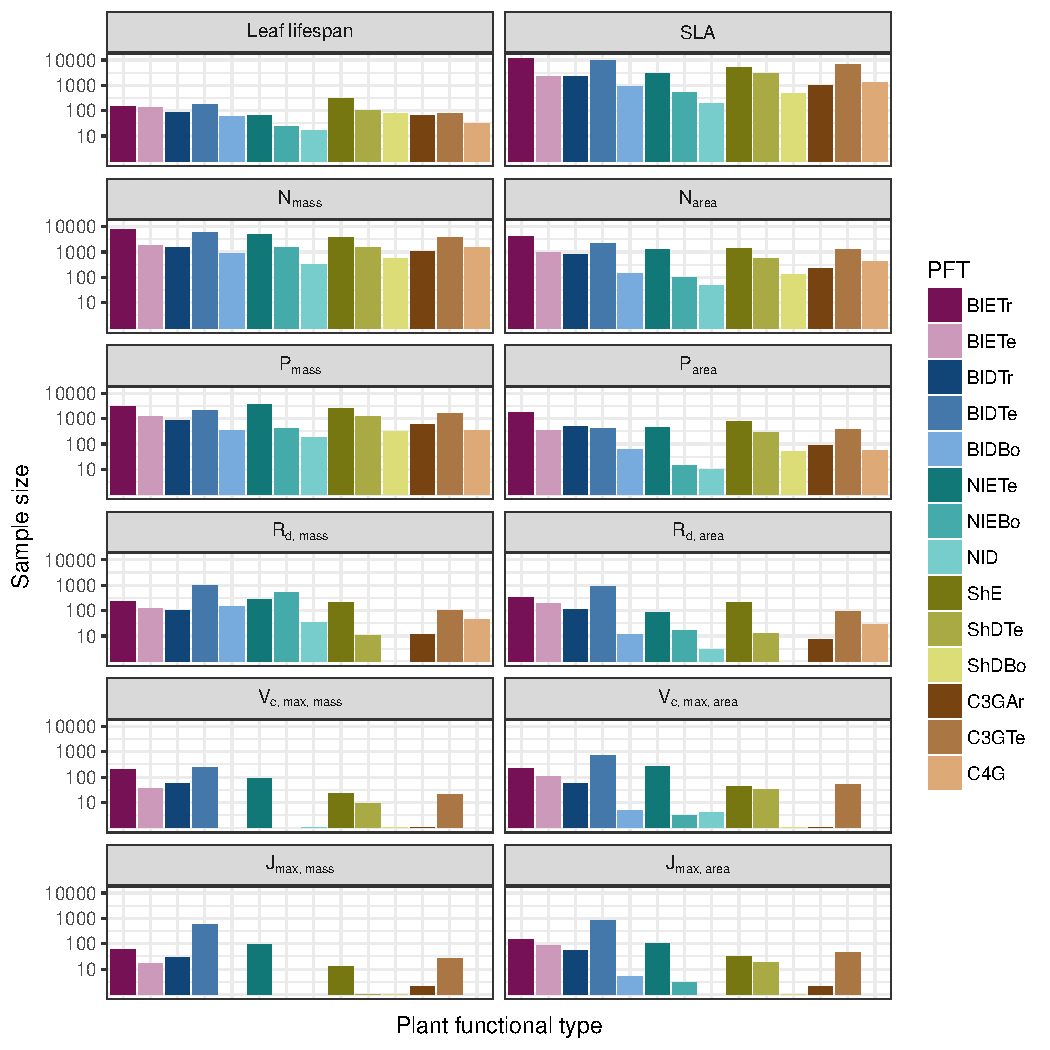
\includegraphics[width=\textwidth]{1_mvtraits/figures/sample_size.pdf}
  \caption{%
    Sample sizes for each trait-PFT pair. $y$ axis is scaled logarithmically.
  }\label{fig:mvtraits-fig1}
\end{figure}


\subsection{Multivariate analysis}

\subsubsection{Basic model description}

In this study, we compared three different models representing different levels of complexity.

The simplest model was the ‘univariate’ model, in which each trait was modeled independently.
For an observation $x_{i,t}$ of trait $t$ and sample $i$:

\[x_{i,t} \sim N(\mu_t, \sigma_t)\]

where $N$ is the univariate normal (Gaussian) distribution with mean $\mu_t$ and standard deviation $\sigma_t$ for trait $t$.

The second-simplest model was the ‘multivariate’ model, in which traits were modeled as samples from a multivariate distribution with a single mean vector and covariance matrix.
For the observed vector of traits ${\mathbf{x_i}}$ for sample $i$:

\[\mathbf{x_i} \sim mvN(\mathbf{\mu}, \mathbf{\Sigma})\]

where $mvN$ is the multivariate normal (Gaussian) distribution with mean vector $\mathbf{\mu}$ and variance-covariance matrix $\mathbf{\Sigma}$.
We ran both of these models independently for each PFT as well as for the entire dataset (as if every observation belonged to the same PFT).

The most complex model was the ‘hierarchical’ model, in which observed trait values were drawn from a PFT-specific multivariate normal distribution describing within-PFT variation and whose parameters were themselves sampled from a global multivariate distribution describing the variation across PFTs.
For the observed vector of traits $\mathbf{x}_{i,p}$ for sample $i$ belonging to PFT $p$:

\[\mathbf{x}_{i,p} \sim mvN(\mathbf{\mu}_p, \mathbf{\Sigma}_p)\]
\[\mathbf{\mu}_p \sim mvN(\mathbf{\mu}_g, \mathbf{\Sigma}_g)\]

where $\mathbf{\mu}_p$ and $\mathbf{\Sigma}_p$ are the mean vector and variance-covariance matrix describing variation within PFT $p$, and $\mathbf{\mu}_g$ and $\mathbf{\Sigma}_g$ are the mean vector and variance-covariance matrix describing across-PFT (global) variation.


\subsubsection{Model implementation}

We fit the above models using a Gibbs sampling algorithm that leveraged known conjugate prior relationships for efficient exploration of the sampling space.
For priors on all multivariate mean vectors ($\mathbf{\mu}$), we used normal distributions:

\[P(\mathbf{\mu}) \sim mvN(\mathbf{\mu}_0, {\mathbf{\Sigma}}_0)\]

This gives rise to the following expression for the posterior:

\[P(\mathbf{\mu} \mid 
    \mathbf{x}, \mathbf{\Sigma}, 
    \mathbf{\mu}_0, \mathbf{\Sigma}_0)
  \sim
  mvN(\mathbf{\mu^*}, \mathbf{\Sigma^*})\]

\[\mathbf{\Sigma^*} = {(\mathbf{\Sigma}_0^{-1} + n \mathbf{\Sigma}^{-1})}^{-1}\]
\[\mathbf{\mu^*} = \mathbf{\mu}_0 \mathbf{\Sigma}_0^{-1} + \bar{\mathbf{x}} n \mathbf{\Sigma}^{-1}\]

where ${\bar{{\mathbf{x}}}}$ are the sample means of the data and $n$ is the number of rows in the data.

For priors on all multivariate variance-covariance matrices, we used the Wishart distribution ($W$):

\[P(\mathbf{\Sigma}) \sim W(\nu_0, \mathbf{S}_0)\]

This gives rise to the following expression for the posterior:

\[P(\mathbf{\Sigma} \mid
  \mathbf{x}, \mathbf{\mu},
  \nu_0, \mathbf{\Sigma}_0)
  \sim
  {(W(\nu^*, S^*))}^{-1}\]

\[\nu^* = 1 + \nu_0 + n + m\]
\[\mathbf{x^*} = \mathbf{x} - \bar{\mu}\]
\[\mathbf{SS} = \mathbf{x^*}^{T} \mathbf{x^*}\]
\[\mathbf{S^*} = {(\mathbf{S}_0 + \mathbf{SS})}^{-1}\]

where $n$ is the number of rows and $m$ is the number of columns in data matrix $x$~\cite[full derivation in][]{gelman_bayesian}.

The fundamentally multivariate nature of the sampling procedure described above makes it incapable of accommodating partially missing observations.
Therefore, our algorithm also included imputation of partially missing data, which proceeded as follows:
For a block of data $\mathbf{x'}$ containing missing observations in columns $\mathbf{m}$ and present observations in columns $\mathbf{p}$,
the missing values $\mathbf{x'}[m]$ are drawn randomly from a conditional multivariate normal distribution at each iteration of the sampling algorithm:

\[\mathbf{x'}[m|p] \sim mvN(\mathbf{\mu}', \mathbf{\Sigma}')\]

\[\mathbf{\mu'} = 
  (\mathbf{x'}[p] - \mathbf{\mu'}[p]) 
  ({\mathbf{\Sigma}[p,p]}^{-1} \mathbf{\Sigma}[p,m])\]
\[\mathbf{\Sigma'} = \mathbf{\Sigma}[m,m] - 
  \mathbf{\Sigma}[m,p]
  ({\mathbf{\Sigma}[p,p]}^{-1} \mathbf{\Sigma}[p,m])\]

For each model fit, we ran five parallel MCMC chains, continuing the sampling until the final result achieved convergence as determined by a Gelman-Rubin potential scale reduction statistic less than 1.1~\cite{gelman_1992_inference}.
We implemented this sampling algorithm in an open source, publicly available R~\cite[version 3.4.3,][]{rstats} package (\texttt{http://github.com/ashiklom/mvtraits}).


\subsubsection{Analysis of results}

To assess the impact of multivariate and hierarchical constraint on trait estimates,
we compared the mean and 95\% confidence intervals of trait estimates for each PFT from each model (Fig.~\ref{fig:mvtraits-fig2}).
For reference, we also added the default parameter values of CLM 4.5~\cite[Table 8.1 in][]{clm45_note} for SLA, $N_{\mass}$, $N_{\area}$, $V_{c,\max,\mass}$, and $V_{c,\max,\area}$ to Fig.~\ref{fig:mvtraits-fig2}.
To convert CLM's reported C:N ratio to $N_{\mass}$, we assumed a uniform leaf C fraction of 0.46.
We then divided this calculated $N_{\mass}$ by the reported SLA to obtain $N_{\area}$.
We calculated $V_{c,\max,\mass}$ by multiplying the reported $V_{c,\max,\area}$ by the reported SLA\@.

To test the hypothesis that the multivariate and hierarchical models offer more value in terms of uncertainty constraint at smaller sample sizes, we calculated the relative uncertainty ($\alpha$) as a function of the mean ($\mu$) and upper ($q_{0.975}$) and lower ($q_{0.025}$) confidence limits of trait estimates.

\[ \alpha = \frac{q_{0.975} - q_{0.025}}{\mu} \]

We then fit a generalized linear model relating relative uncertainty to sample size ($n$) for each of the model types (univariate, multivariate, and hierarchical; Fig.~\ref{fig:mvtraits-fig3}).

\[ \log{\alpha} = b_0 + b_1 \log{n} \]

If all three models performed equally well at all sample sizes, their respective slope and intercept coefficients would be statistically indistinguishable.
On the other hand, models that perform better should have
lower intercept ($b_0$) coefficients, indicating generally lower uncertainty,
and
lower slope ($b_1$) coefficients, indicating a reduced sensitivity of uncertainty ($\alpha$) to sample size ($n$).

To assess the consistency of within- and across-PFT trait trade-offs, we looked at covariance estimates for each trait pair and, where these values were significantly different from zero ($p < 0.05$),
we calculated the eigenvalues from the pairwise variance-covariance matrix for that trait pair and plotted the corresponding dominant eigenvectors centered on the mean estimates (Fig.~\ref{fig:mvtraits-fig4}).
This figure provides a visual representation of relative positions of PFTs in trait space and both the direction and extent of within-PFT trait covariance, and is directly analogous to conceptual figures describing hierarchical trait variability across environmental gradients as presented in, for instance,~\cite{cornwell_community_2009} and~\cite{albert_intraspecific_2010}.
Due to the small number of points used to estimate across-PFT covariance in the hierarchical model, none of the across-PFT covariances estimated in the hierarchical model were significantly different from zero ($p < 0.05$).
For this reason, we compared within-PFT covariances as estimated by the hierarchical model with the covariances estimated by fitting a multivariate model to all of the data.

Besides the consistency in the direction of trait covariance globally and between different PFTs, we also investigated the strength and predictive power of these covariances, which is represented by correlation coefficients (i.e.\ the pairwise covariance normalized to the variances of the component variables).
To do this, we plotted the mean and 95\% confidence interval of the pairwise trait correlation coefficients for the global estimate from the pooled multivariate model and PFT-level estimates from the hierarchical model (Fig.~\ref{fig:mvtraits-fig5}).

The R code and ancillary data for running these analyses is publicly available online via the Open Science Framework (OSF) at \texttt{https://osf.io/w8y73/}.
The TRY data used for this analysis can be requested at \texttt{http://try-db.org}.
